\section{Primární aktivity}

Z celé množiny funkcionalit \gls{is} lze vyčlenit několik primárních aktivit, na které budou uživatelé klást největší důraz při práci. Dané činnosti, vzhledem k jejich důležitosti, jsou znázorněny do \gls{uml} diagramů aktivit nebo podrobně zanalyzovány.


% --------------------------------------------------------------------------------------------------
% Autentizace
% --------------------------------------------------------------------------------------------------


\subsection{Autentizace uživatelů}

Základní a prvotní činností \gls{is} je registrace či následné přihlášení neautentizovaných uživatelů. Vzhledem k absenci vlastního autorizačního serveru jsou využívány autorizační servery třetích stran.

Cyklus autentizace přes vybraný servis~\ref{pic:dia-ak-auth} začíná uživatelským požadavkem na server. Informační systém přesměruje uživatele na stránky třetí strany, kdy v případě první návštěvy bude uživatel dotázán na povolení poskytovaní jistých osobních informací. V případě odmítnutí je ukončen celý proces autentizace. Pokud uživatel povolil poskytování informací, nebo ho již měl schválený, tak autorizační server posílá potřebná data na server \gls{is}.

Dle poskytnutých informací server ověřuje, zda se jedná o nového uživatele, pak zakládá nový účet se všemi náležitostmi (přiřazení výchozí role, oznámení, apod.), nebo o již existujícího, potom kontroluje, zda není potřeba aktualizovat některé informace vzhledem k údajům (údaje, které nemají přímý vliv na identifikaci -- jméno, email, apod.).

Po vytvoření, či aktualizaci databáze se vytváří unikátní autorizační klíč, jenž je následně předán klientské aplikaci. Tento klíč je uložen je uložen na klientovi a používán v případě autorizovaných požadavků na server.


\begin{fig:illustration}
   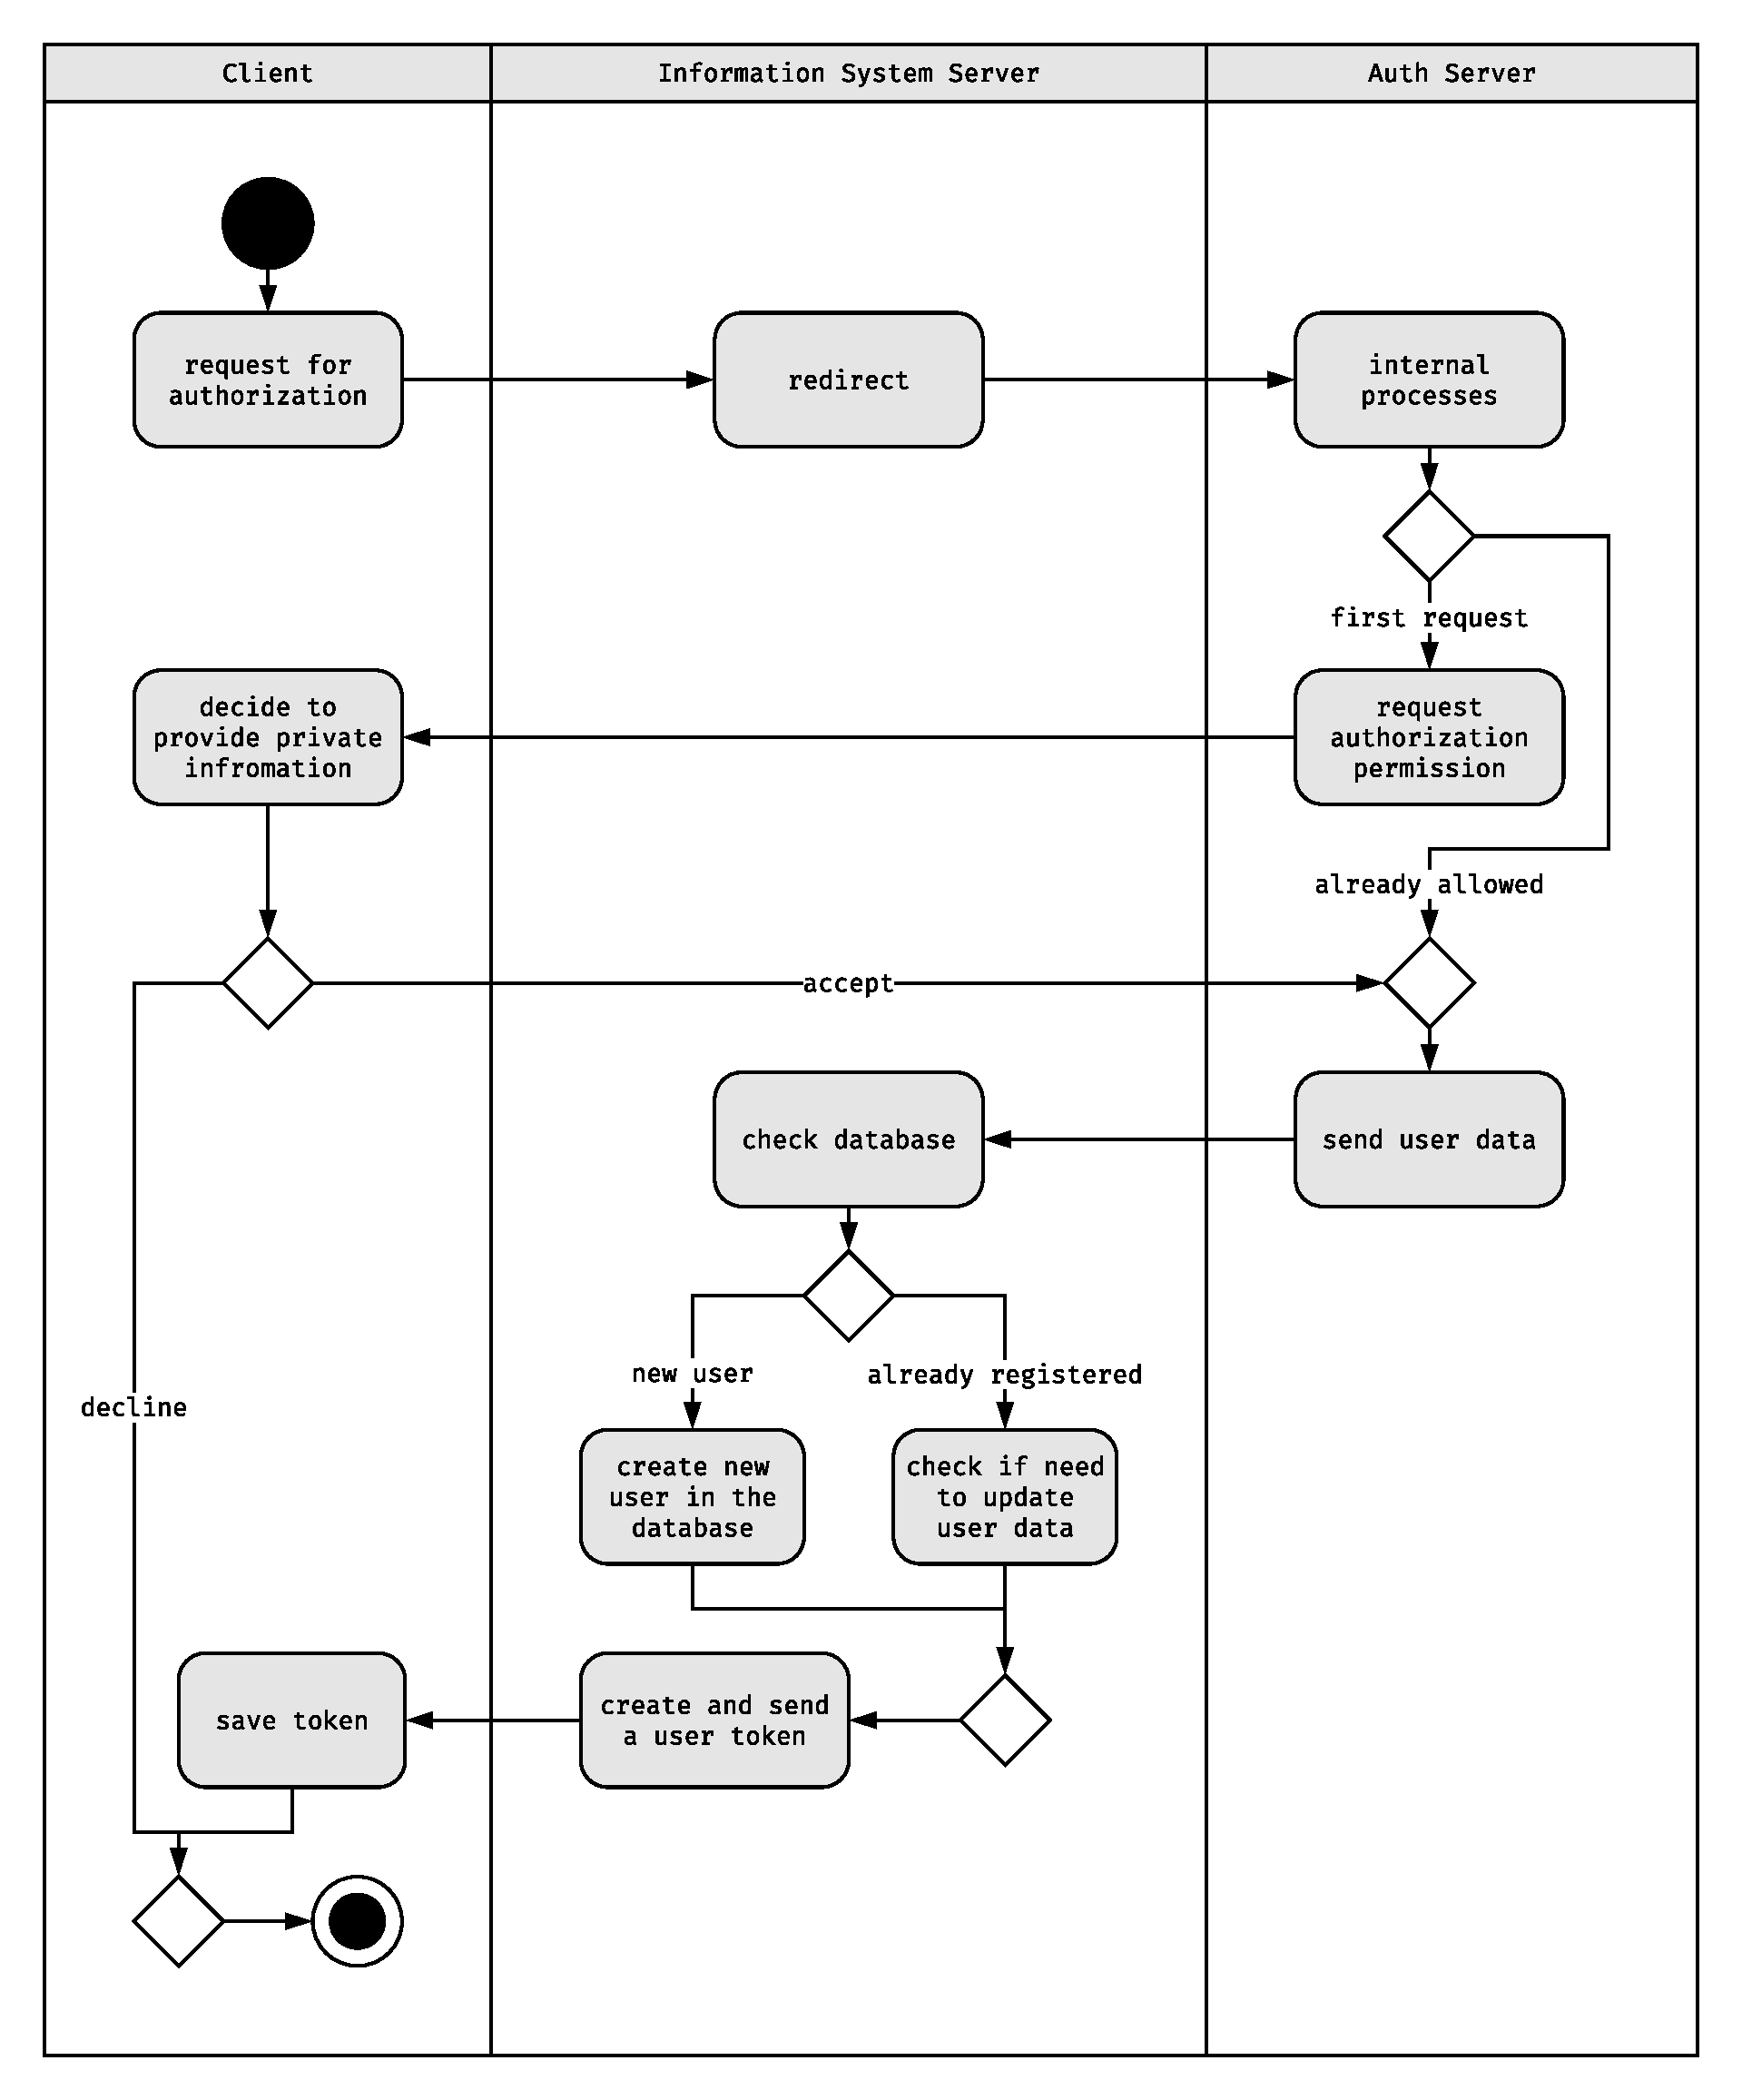
\includegraphics[width=1\textwidth]{images/dia-ak-auth.pdf}
   \caption[Diagram procesu autentizace]{Diagram procesu autentizace}\label{pic:dia-ak-auth}
\end{fig:illustration}


% --------------------------------------------------------------------------------------------------
% Správa projektu
% --------------------------------------------------------------------------------------------------


\subsection{Správa obsahu projektu}

Hlavním cílem projektového týmu bude tvorba obsahu pro plnění úkolů v iteracích. Obsah se skládá z jednotlivých částí, které uchovávají svoje data -- samotný text či jiné informace, název šablony, jenž bude v předem definované podobě zobrazovat informace části uživateli, a seznam úkolů, které tato část splňuje. 

Vznik a správa částí je plně řízena vedoucími a spolupracovníky projektu. Návštěvníci a jiní uživatelé mohou pouze zobrazit obsah (pokud na to mají právo dle globální role a nastavení projektu).

V dané specifikaci všechny části mají být nezávislé, ale pro budoucí rozvoj je třeba počítat se snadno rozšiřitelnou strukturou, aby se dala nastavit výměna dat ve sdíleném úložišti. Celkový průběh generování obsahu popisuje diagram \ref{pic:dia-ak-content} -- po požadavku uživatele zobrazit obsah jsou staženy části projektu do prohlížeče a zanalyzovány. Na základě analýzy vzniká seznam potřebných šablon, které jsou rovněž staženy ze serveru a následně použity pro generování obsahu z dat každé části. V případě chybějící nebo jinak poškozené šablony či dat části je zobrazena chyba.

\begin{fig:illustration}
   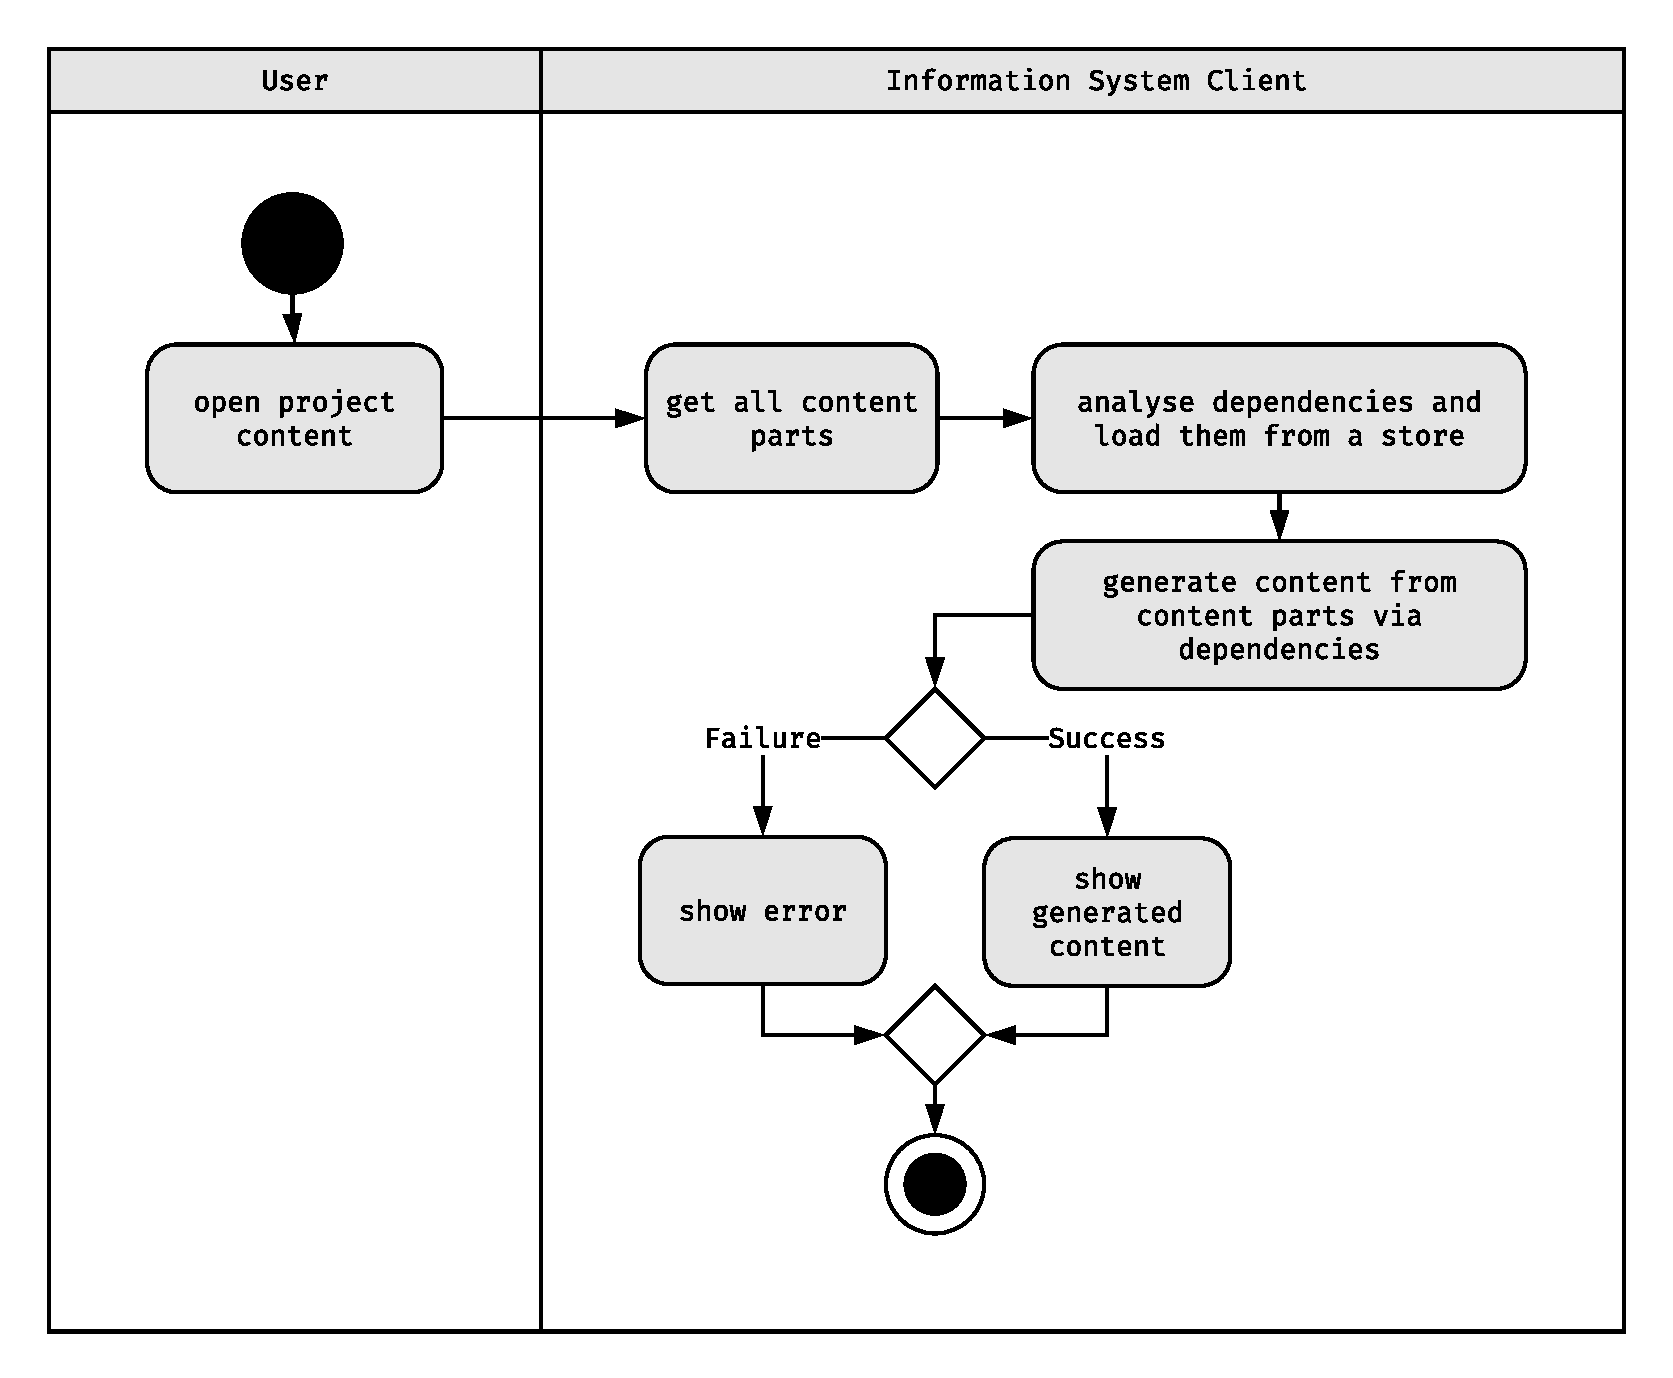
\includegraphics[width=1\textwidth]{images/dia-ak-content.pdf}
   \caption{Diagram generování obsahu projektu}\label{pic:dia-ak-content}
\end{fig:illustration}


% --------------------------------------------------------------------------------------------------
% Vyhledávání projektů
% --------------------------------------------------------------------------------------------------


\subsection{Vyhledávání projektů}

Pro většinu uživatelů veškerá činnost v \gls{is} bude začínat vyhledáváním potřebného projektu. Důvodem může být pokračování v tvorbě obsahu, snaha se připojit k existujícímu týmu, zobrazení existujících dat, apod. Z uživatelského hlediska je vhodné mít pro všechny případy vyhledávání dva základní seznamy:

\begin{ulnar}
   \item seznam se všemi veřejně přístupnými projekty
   \item seznam projektů, v nichž je uživatel uveden jako účastník
\end{ulnar}

Seznam přístupných projektů bude určen především pro vyhledávání cizích projektů a dle předpokladu bude méně využívaný, než seznam s uživatelskými projekty. Filtrování obou seznamů bude založeno na volbě obecných vlastností:

\begin{ulnar}
   \item kategorie,
   \item jméno projektu,
   \item stav archivace,
   \item důvěryhodnost (majitel projektu je důvěryhodný),
   \item stav volného přihlašování do projektu,
   \item projekty, do kterých má uživatel přístup,
   \item projekty, ve kterých je uživatel vedoucím.
\end{ulnar}

Následně však může být upřesněno filtrováním dle volitelných štítků. Zavádění podkategorií nebo jiných přesně stanovených seznamů je nevhodné, protože by omezovalo uživatelskou činnost. Štítky představují volnou formu klíčových slov. Jsou ukládány při prvním použití a následně nabízeny všem uživatelům během upravování štítků.


% --------------------------------------------------------------------------------------------------
% Nabídka pozic
% --------------------------------------------------------------------------------------------------



\subsection{Nabídka pozic}

Poslední aktivitou, na kterou bude kladen důraz v \gls{is}, je týmová práce a nabídka vakantních míst. Diagram aktivit~\ref{pic:dia-ak-role-assing} zachycuje průběh náboru vývojářského týmu. Nejdřív vedoucí definuje vakantní pozice, které jsou potřeba do projektového týmu a jejich kapacitu (například 5 volných míst pro vývojáře). Po otevření volného přihlašování do rolí se čeká, až uživatelé najdou projekt, projeví zájem o jednu z daných pozic a odešlou požadavek, že se o danou roli chtějí ucházet. \gls{is} se pokusí začlenit uživatele do týmu. V případě, že už je součástí projektu, tak pouze změní roli.


\begin{fig:illustration}
   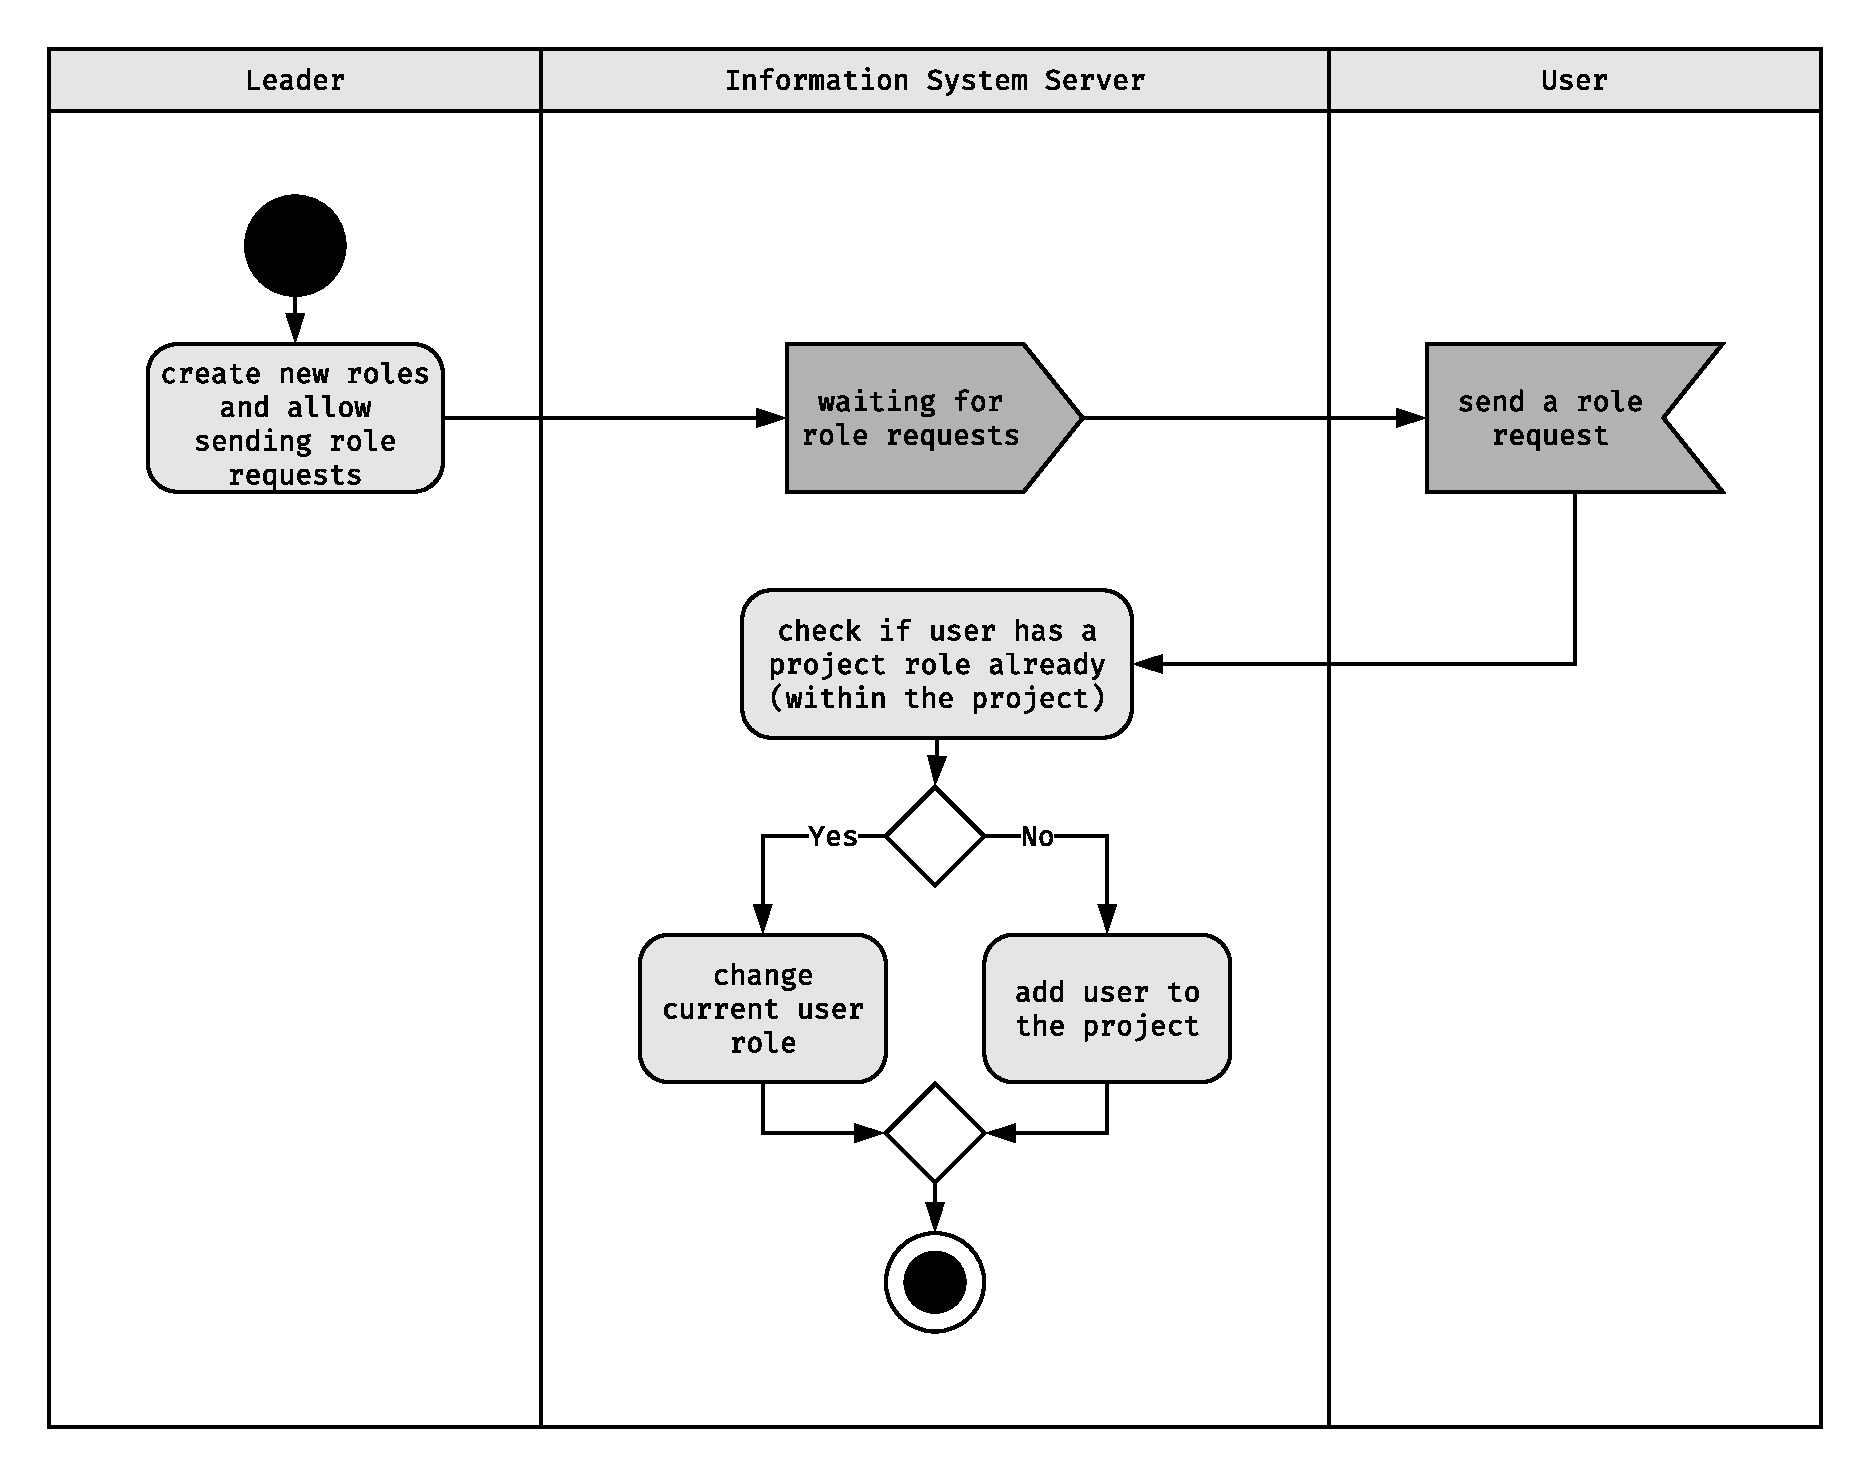
\includegraphics[width=1\textwidth]{images/dia-ak-role-assing.pdf}
   \caption[Diagram průběhu náboru týmu]{Diagram průběhu náboru vývojářského týmu}\label{pic:dia-ak-role-assing}
\end{fig:illustration}


Daný proces přiřazování projektové role uživateli mohou ignorovat vedoucí projektů se statusem důvěryhodného účastníka systému. Mají právo přidávat uživatelé do vlastních projektů bez jejich souhlasu. V tomto případě rovněž neplatí omezení kapacity rolí.
